
\documentclass{article}
\usepackage{marvosym}


\input /Users/vigon/visible/MesRacoursis2015



\title{Le calcul stochastique d'Ito}


% Mettre à 1 pour cacher les parties, à 0 pour les faire apparaitre. 
\definecolor{cache}{gray}{1}
%COMMENTER LES DEUX LIGNES SUIVANTES POUR ajouter LES PARTIES ENCADREES
\def\pournous{\comment} 
\def\endpournous{\endcomment}


\begin{document}
\maketitle


    



\section{Généralités}


\subsection{Filtration}

La variable $t\in \co R_+$ représente le temps. Le plus souvent, nous la mettons en indice. ex: $X_t =X(t)$.  

On considère une "filtration"  $(F_t)_{ t\geq 0}$.  C'est une suite d'objets aléatoires vérifiant : 
 $$
 \fo s<t \qq \ex fonc  : \qq F_s=fonc(F_t) \eqno{(Fil)} 
 $$
 L'objet $F_t$ représente  toute l'information connue à l'instant   $t$.   L'hypothèse ci-dessus nous indique  qu'au temps $t$ on connait aussi l'information du temps $s$. On a donc de la mémoire.

Exemple : dans un cadre de la simulation, $F_t$ représente tous les résultats des rand() que nous avons lancé de $0$ à $t$. 


On appellera trajectoire\footnote{le terme technique est "processus adapté" } les fonctions de $\co R^+$ dans $\co R^n$ telle que pour tout $t$, $X_t$ est une fonction de $F_t$.   En particulier  $X_t$ n'a pas le droit d'être défini à partir de $F_{t+1}$. Moralement,  les trajectoires n'anticipent pas le futur (elles sont "adaptées" à la filtration $F_t$).


\subsection{Mouvement brownien dans une filtration}

On appellera mouvement brownien dans la filtration $F_t$ une trajectoire $W_t$ telle que 
\begin{itemize}
\item $t \to W_t$ est continue. 
\item pour tout $s,t$, $W_{t+s}-W_t$ est indépendant de $F_t$. \ \ \ \   (donc indépendant de $W_t$ car $W_t=fonc(F_t)$).
 \item pour tout $s,t$, $W_{t+s}-W_t$ suit une loi normale centrée de variance $s$. 
\end{itemize}
 Remarque :  les mouvements browniens sont aussi appelés "processus de Wiener", d'où la lettre $W$.  Mais cette lettre nous rappelle aussi qu'ils oscillent beaucoup.  En particulier ils ne sont pas dérivables (vous observerez les simulations). 


\subsection{Mouvement brownien tout court}

On peut aussi définir un brownien  sans parler de filtration :  $W$ est un mouvement brownien (tout court) lorsque
\begin{itemize}
\item $t \to W_t$ est continue. 
\item pour tout $s,t$, $W_{t+s}-W_t$ est indépendant de $W_{[0,t]}$ (càd tout le bout de trajectoire de 0 à t).
 \item pour tout $s,t$, $W_{t+s}-W_t$ suit une loi normale centrée de variance $s$. 
\end{itemize}
Ce qui est équivalent à dire que $W_t$ est un brownien dans la filtration $F_t :=W_{[0,t]}$ (c'est la filtration naturelle du passé de $W_t$). 

Ainsi on a plusieurs cadres de travail possibles
\begin{itemize}
\item   cadre simple : on se donne un brownien $W_t$ (tout court) et on considère la filtration $F_t= W_{[0,t]}$. Cela vérifie l'hypothèse $(Fil)$ car 
$$
\fo s<t : \qq W_{[0,s]} = \Big(W_{[0,t]} \Big)_{[0,s]}
$$
\item cadre complexe : on se donne une filtration $F_t$ qui englobe tous les browniens et autres trajectoires que l'on veut considérer. 
\end{itemize}



Remarque :   
\begin{itemize}
\item Dans les livres, le plus souvent, les filtrations sont des suites de "tribus", mais cela revient strictement au même. 
\item Dans la suite, nous supposons aussi que la filtration $t\to F_t$ est continue : l'information croît sans accoup.     Cette hypothèse est vérifiée "intuitivement" quand on prend $F_t=W_{[0,t]}$
\item Le calcul stochastique que nous présentons n'est pas du tout adapté aux processus stables que nous avons simulé. Nous avons observé qu'ils sautaient brutalement : ils ne peuvent donc pas s'adapter à une filtration continue. Le calcul stochastique pour des processus avec saut existe, mais les formules sont bien plus compliquées. 
\end{itemize}

\section{Equation différentielle}

\subsection{Simple}
 
Considérons une trajectoire $a_t$.  L'équation différentielle
 $$
   \frac {dX_t}{dt}   =a_t  
  $$
 s'écrit plus joliment
 $$
 dX_t = a_t \, dt
 $$
s'interprète ainsi :  
$$
X_{t+ \ep } -X_t = a_t \ep
$$
 se résout approximativement avec le schéma d'Euler : on se donne un point de départ $x_0$ et une suite de temps $t_i$ très serrés et l'on pose 
$$
X_{t_{i+1}} = X_{t_i} +    a_{t_i} (t_{i+1} -t_i) 
$$




\subsection{Avec une autre trajectoire}

Considérons des trajectoires $a_t,b_t,Y_t$ avec $Y_t$ dérivable.  L'équation différentielle
$$
 \frac {dX_t}{dt} = a_t  + b_t \frac {dY_t}{dt}
 $$
 s'écrit plus joliment
$$
 dX_t = a_t \, dt + b_t dY_t 
 $$
s'interprète ainsi :  
$$
X_{t+ \ep } -X_t = a_t \ep + b_t (Y_{t+\ep}-Y_t) 
$$
se résout approximativement avec le schéma d'Euler : on se donne un point de départ $x_0$ et une suite de temps $t_i$ très serrés et l'on pose 
$$
X_{t_{i+1}} =  X_{t_i} +    a_{t_i} (t_{i+1} -t_i)   + b_{t_i} (Y_{t_{i+1}}- Y_{t_i}) 
$$


\subsection{Avec une excitation brownienne}

Considérons des trajectoires $a_t,b_t$ et une trajectoire brownienne $W_t$.  Le brownien n'étant pas dérivable, on n'écrira PAS
$$
 \frac {dX_t}{dt} = a_t  + b_t \frac {dW_t}{dt}
 $$
 Mais on écrit quand même une "équation différentielle stochastique" :
$$
 dX_t = a_t \, dt + b_t dW_t 
 $$
Elle s'interprète ainsi :  
$$
X_{t+ \ep } -X_t = a_t \ep + b_t (W_{t+\ep}-W_t) 
$$
Donc : les accroissements infinitésimaux de $X_t$ dépendent des accroissements infinitésimaux du Brownien. On dit que $X_t$ subit une excitation brownienne.  L'équation différentielle stochastique se résout grâce au schéma d'Euler :
$$
X_{t_{i+1}} =  X_{t_i} +    a_{t_i} (t_{i+1} -t_i)   + b_{t_i} (W_{t_{i+1}}- W_{t_i}) 
$$
Nous  programmerons ce schéma en TP. 




\subsection{Où intervient la tribu $F_t$}

Pour résoudre les équations différentielles, nous utilisons le schéma d'Euler, par exemple :  
$$
X_{t_{i+1}} =  X_{t_i} +    a_{t_i} (t_{i+1} -t_i)   + b_{t_i} (W_{t_{i+1}}- W_{t_i}) 
$$
Ainsi, quand nous sommes à l'instant $t_i$, pour construire $X_{t_{i+1}}$, nous avons besoin de connaitre le triplet $X_{t_i},a_{t_i},b_{t_i}$... Et nous les connaissons !  puisque se sont des fonctions de l'ensemble de nos connaissances $F_{t_i}$.  Nous avons aussi besoin  de simuler l'accroissement brownien $(W_{t_{i+1}}- W_{t_i}) $... Et il est facile à simuler ! puisqu'il est indépendant de $F_{t_i}$, donc indépendant du triplet $X_{t_i},a_{t_i},b_{t_i}$


Contre-exemple : L'équation différentielle
$$
dX_t =   X_{t+ 10} dW_t
$$
est impossible à résoudre (notre schéma d'Euler ne fonctionne pas). A chaque instant $t_i$, nous avons besoin de connaitre $X_{t_i + 10}$ que nous n'avons pas encore construit. Par contre
$$
dX_t = X_{t-10} dW_t
$$
fonctionne (en supposant par exemple que $X_{t-10}=X_0$ quand $t<10$). 
 
 
 

\subsection{Trajectoire régulière et excitée}



Fixons le vocabulaire pour la suite :
\begin{itemize}
\item Une trajectoire  $X_t$ est dite régulière lorsqu'il existe un trajectoire $a_t$ telle que
$$
dX_t = a_t dt
$$
Ce qui est équivalent au fait que
$$
X_t = X_0 + \int_0^t a_s ds 
$$
Cela implique notamment que $X_t$ est dérivable presque partout, avec  $a_t$ comme dérivée. 
\item Une trajectoire $X_t$ est dite excitée\footnote{Le terme technique est "semi-martingale"}  lorsqu'il existe des trajectoires $a_t,b_t$ et un  mouvement brownien $W_t$ tel que
$$
dX_t= a_t dt + b_t \, dW_t 
$$
Les trajectoires régulières sont des cas particuliers des trajectoires excitées ($b_t=0$). Mais quand $b_t$ n'est pas partout nul, alors une trajectoire excitée hérite de la non-dérivabilité du brownien. 
\end{itemize}

 
\section{Chain-rule}

En français, la "chain-rule" est la "règle de dérivation composée".

\subsection{La chain-rule pour les trajectoires régulières}

Considérons maintenant une fonction $f(x)$ de  $\co R$ dans $\co R$.  Notons $f'$ et $f''$ ses dérivées premières et secondes.
Quand $X_t$ est une trajectoire régulière nous avons : 
$$
\frac {d f(X_t)}{dt} = f'(X_t)      \frac{dX_t}{dt} 
$$
qui s'écrit plus joliment :  
$$
d f(X_t) = f'(X_t) \, dX_t 
$$
Cette formule est {\bf fausse} quand $X_t$ est une trajectoire excitée.


\subsection{Le crochet stochastique}

Le crochet stochastique est un produit scalaire sur les accroissements différentiels (on verra plus loin une définition). Il est donc symétrique :
$$
\cc dX_t , dZ_t\bb=\cc  dZ_t, dX_t\bb
$$
Linéaire :
$$
\cc dX_t + dY_t, dZ_t\bb  = \cc dX_t , dZ_t\bb+\cc dY_t, dZ_t\bb
$$
Les éléments non différentiel sortent comme des constantes
$$
 \cc a_t\, dX_t , dZ_t\bb  =a_t\,  \cc  dX_t , dZ_t\bb
$$
Dès qu'un des éléments est réduit à $dt$, le crochet s'annule
$$
\cc dX_t, dt\bb =0 
$$
Si les deux éléments sont des Browniens indépendants alors le crochet s'annule
$$
\cc dW_t, d\tilde W_t  \bb =0 
$$
mais s'il y a le même brownien des deux côtés alors :
$$
\cc dW_t, d W_t  \bb = dt
$$


Exemples quand $dX_t = a_t dt +  b_t  dW_t + c_t d\tilde W_t$ et $d Y_t = i_t dt + j_t dW_t + k_t d\tilde W_t$ alors
\begin{alignat*}{1}
\cc dX_t, d \tilde Y_t   \bb = b_t j_t \, dt + c_tk_t \, dt
\end{alignat*}


\subsection{Chain rule pour les trajectoires excitées}


\begin{theoreme}[Formule d'Ito] Considérons $X_t$ une trajectoire excitée. Considérons $f$ une fonction deux fois dérivables, on a 
$$
df(X_t) = f'(X_t) dX_t   +   \frac 1 2 f''(X_t) \, \cc dX_t,dX_t\bb
$$
\end{theoreme}
En particulier si $dX_t =a_t dt + b_t dW_t$ : 
$$
df(X_t) = f'(X_t) dX_t   +   \frac 1 2 f''(X_t)  b_t^2 \, dt
$$
Retenez bien ce terme supplémentaire dans la chain-rule.  
Remarquez que lorsque $X_t$ est une trajectoire régulière, le crochet différentiel s'annule et on retombe sur la chain-rule-régulière. 


\subsection{Exemples}

\begin{itemize}
\item Essayons de définir une trajectoire excitée qui vérifie $$dX_t = X_t dW_t$$ (nous verrons l'intérêt dans la partie math financière).  En vieux routier du calcul diff, on va essayer de résoudre cette équation en posant $X_t = e^{W_t}$. Mais la chain-rule-excitée nous donne :
$$
d  (e^{W_t})  =  e^{W_t}   dW_t + \frac 1 2   e^{W_t} dt = X_t (dW_t + \frac 1 2 dt  )
$$ 
Raté ! 
\item Montrez que c'est $X_t = e^{W_t - \frac 1 2 t}$ qui satisfait $dX_t = X_t dW_t$. 
\item Prenez une trajectoire excitée $dX_t = a_t dt + b_t dW_t$. Quelle équation différentielle vérifie $X^2_t, \ln X_t , e^{X_t}$ ?
\end{itemize}



\subsection{Explication}

Rappelons le développement de Taylor
$$
f(x+\ep) = f(x) + f'(x) \ep + \frac 1 2 f''(x) \ep^2 + ... 
$$


Soit $X_t$  une trajectoire régulière. En utilisant le développement de Taylor à l'ordre 1 on a 
$$
f(X_{t+\ep})  - f(X_t )  = f'(X_t)  (X_{t+\ep}-X_t )  +  o(  X_{t+\ep} -X_t  ) 
$$
Et en passant à la limite le reste à l'ordre 1 est négligeable devant les autres termes ce qui donne
$$
df(X_t) = f'(X_t) dX_t 
$$
Quand $X_t$ est une trajectoire excitée, le reste à l'ordre 1 n'est pas négligeable et il faut effectuer Taylor à l'ordre 2 :  
$$
f(X_{t+\ep})  - f(X_t )  =  f'(X_t)  (X_{t+\ep}-X_t )  +   \frac 12 f'' (X_t)  ( X_{t+\ep} -X_t )^2  +    o( X_{t+\ep} -X_t )^2 
$$
Qui donne à la limite
$$
df(X_t) =  f'(X_t) dX_t   +   \frac 1 2 f''(X_t) \, \cc dX_t, dX_t \bb
$$
Le crochet stochastique étant  défini comme étant la limite, en un certain sens, de $ (X_{t+\ep} -X_t )^2$.







\section{Intégrales d'Ito}


\subsection{Dualité intégration/dérivation}
Une trajectoire régulière est définie par une équation différentielle  et un point de départ :
$$
\begin{cases}
dX_t = a_t \, dt \\
X_0=x_0
\end{cases}
 $$
Mais cette même trajectoire peut être définie par :
$$
X_t = x_0 +  \int_0^t a_s \, ds 
$$
où $\int_0^t$ est l'intégrale usuelle ;  que l'on peut construire avec la formule des rectangles, des trapèzes, ou encore en utilisant le cadre théorique de l'intégrale de Lebesgues.  

Cela nous rappelle qu'il y a deux manières de présenter "dérivation" et "intégration" :
\begin{itemize}
\item L'opération de dérivation peut être définie comme l'opération inverse de l'opération primitive (qui se construit elle même avec la notion d'intégrale). 
\item L'opération primitive (et donc la notion d'intégrale)  peut être définie comme l'opération inverse de la dérivation.
\end{itemize}


\subsection{L'intégrale d'Ito}

Une trajectoire excitée est définie par une équation différentielle stochastique et un point de départ :
$$
\begin{cases}
dX_t =  a_t \, dt + b_t \, dW_t \\
X_0=x_0
\end{cases}
 $$
On aimerait aussi pouvoir la définir comme ceci :
$$
X_t = X_0 + \int_0^t a_s ds  + \int_0^t b_s dW_s 
$$
Il faut donc donner un sens à la seconde intégrale :  On  utilise pour cela la formule des rectangles-évalués-à-gauche :  on se donne des temps $(0=s_0^n, s_1^n,s_2^n,...)$ qui se rapprochent quand $n\to \infty$. On définit l'intégrale d'Ito par : 
$$ 
it \!\!\oint_0^t b_s dW_s  : = \lim_n  \sum_{i}   b_{s^n_{i}} ( W_{s^n_{i+1}} - W_{s^n_i} )    1_{s^n_i<t} 
\eqno{(ITO)}
$$

DESSIN

\vspace{3cm}

Si nous remplaçons $W_t$ par une trajectoire régulière $K$, nous retombons sur la notion classique d'intégrale :
\begin{alignat*}{1}
it \!\!\oint_0^t b_s dK_s  & = \lim_n  \sum_{i}   b_{s^n_{i}} ( K_{s^n_{i+1}} - K_{s^n_i} )    1_{s^n_i<t}  \\
& = \lim_n  \sum_{i}   b_{s^n_{i}} \frac {( K_{s^n_{i+1}} - K_{s^n_i} ) }{(s^n_{i+1} - s^n_i) }   (s^n_{i+1} - s^n_i) \ 1_{s^n_i<t}  \\
&= \int_0^t b_s \frac {K_s}{ds}\, ds = \int_0^t b_s \, dK_s 
\end{alignat*}
Puisque l'intégrale d'Ito étend l'intégrale normale, nous la notons simplement $\int$.  On a défini l'intégrale d'Ito par rapport à une trajectoire brownienne, mais on peut la définir par rapport à n'importe quelle trajectoire excitée, en utilisant la linéarité : 
$$
\int_0^t h_s dX_s = \int_0^t h_s (a_s ds + b_s dW_s)= \int_0^t h_s a_s ds + \int_0^t h_s b_s  \, dW_s
$$
L'intégrale d'Ito est alors l'inverse de la différentielle dont nous parlons : 
$$
d \int_0^t  dX_s=  dX_t       \hb{ et }    \int_0^t dX_s = X_t
$$


\subsection{Exemple}

\begin{itemize}
\item Considérons $X_t$ une trajectoire régulière telle que $X_0=0$. La chain-rule-régulière nous donne   
$d (X_t)^2= 2X_t dX_t$. En intégrant : 
$$
X^2_t =2 \int_0^t X_s dX_s  
$$
\item Considérons $X_t = W_t$ une trajectoire brownienne (qui vérifie aussi $W_0=0$). La chain-rule-excitée donne   $d (W_t)^2 = 2W_t dW_t + dt$.  En intégrant :
$$
W_t^2 - t  =2 \int_0^t W_s dW_s
$$
\item Moralité :  Imaginez que vous gagnez à chaque instant $s$ la somme de $X_s\, dX_s$ ; au temps $t$, la formule pour calculer votre gain cumulé ne sera pas la même si $X_t$ est une trajectoire régulière, ou bien un trajectoire excitée~!   A première vue, cela fait penser à une boutade de mathématique pure.   Mais en fait, les cours de bourse sont très proches de trajectoires excitées, et c'est le calcul d'Ito (donc la chain-rule-excitée)   qui est employé  en pratique dans les calculs financiers (cf. la fin de ce cours).  
\end{itemize}




\subsection{Subtilités}

 Attention il y a des subtilités :  
 \begin{itemize}
  \item  La limite dans $(ITO)$  existe dans un sens faible (dans $L^2$). Mais cela implique que pour une certaine sous-suite $n_i$, la limite existe presque-surement, ce qui nous suffit largement.  
 \item  Changeons très légèrement de formule des rectangles. Utilisons la formule des rectangles-évalués-au-milieu :
 $$
\lim_n  \sum_{i}    \Big(   \frac {b_{s^n_{i}} +  b_{s^n_{i}}}{2}  \Big)  ( W_{s^n_{i+1}} - W^n_{s_i} )    1_{s^n_i<t} 
$$
Si $W$ était une trajectoire régulière, cette limite donnerait la même chose que dans $(ITO)$. Mais le Brownien varie si rapidement que le fait d'évaluer la fonction au milieu des rectangles change le résultat (malgré le fait que la base des rectangles tende vers 0).  La  formule ci-dessus  définit une nouvelle intégrale : l'intégrale de Stratanovich.  Elle nécessite plus d'hypothèse sur $b_t$. La notion de dérivée qui se déduit de intégrale de Stratanovich  donne lieu à une notion de différentielle et une autre chain-rule 
\item  La formule des rectangles-évalués-à-gauche correspond au Schéma d'Euler. En effet  en notant :
$$
L_{t_j}  = \sum_{i=0}^j   b_{s^n_{i}} ( W_{s^n_{i+1}} - W^n_{s_i} )
$$
on a  
$$
L_{t_{j+1}} = L_{t_j} +  b_{s^n_{j}}  ( W_{s^n_{j+1}} - W^n_{s_j} )
$$
L'intégrale de Stratanovich  (et la différentielle associée) correspond à un  schéma  numérique "centré".

\end{itemize}



\section{Multi-dimension}

\subsection{Formule d'Ito multi-dimensionnelle}

On considère  maintenant plusieurs browniens indépendants $W^k_t$ et on définit   plusieurs trajectoires excitées $X^i_t$ par : 
$$
dX^i_t = a^{ik}_t   dt + b_t^{ik} dW_t^k 
$$
En TP, nous construirons des processus de dimension 2 en utilisant 2 browniens indépendants, qui pourront avoir toutes sortes de têtes différentes en fonction des $a_t,b_t$. Par exemple : 

$$
\begin{cases}
dX^1_t= dt + X^1_t dW^1_t \\
dX^2_t= dt + X^1_t dW^2_t  
\end{cases}
$$
\begin{center}
\fbox{
   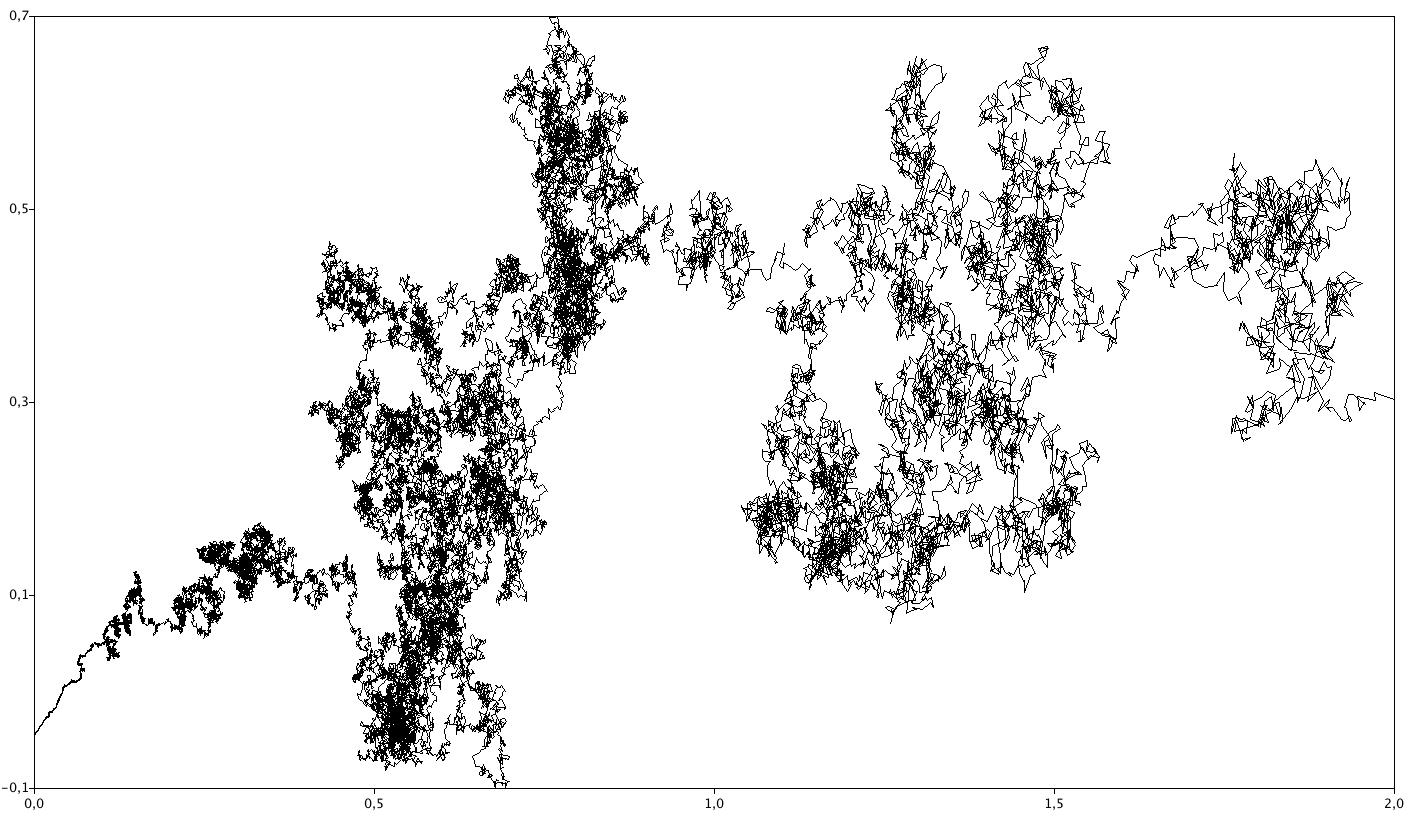
\includegraphics[width=0.5\linewidth]{graph/2.png}
   }
 \end{center}



\begin{theorem}[Formule d'Ito multi-dimensionnelles] Considérons  des trajectoires excitées $(X^1_t,...,X^n_t)$. Considérons $f : \co R^n \to \co R$ une fonction 2 fois dérivable. On a :
$$
d f  (X^1_t,...,X^n_t)  =  \sum_i   \frac {\partial f}{\partial  X_t^i}   \,  dX^i_t    + \frac 1 2  \sum_{ij}    \frac {\partial^2 f}{\partial  X_t^i\partial X_t^j}  \,    \cc dX^i_t, dX^j_t \bb
$$
\end{theorem}




\subsection{Exemples}


\begin{exemple}[Dérivation d'un produit] Considérons 2 trajectoires excitées : 
\begin{alignat}{1}
X_t & = a_t dt +b_t dW_t \\
Y_t &  = c_tdt  + e_t d\tilde W_t 
\end{alignat}
L'opération produit est une fonction : $x\times y = f(x,y)$ que l'on sait bien dériver. Ainsi 
$$
d(X_tY_t) =  X_tdY_t + Y_tdX_t +  \cc dX_t , dY_t \bb   
$$
Ainsi si $W_t=\tilde W_t$ on trouve 
$$
d(X_tY_t) = X_tdY_t + Y_tdX_t + b_te_t dt   
$$
Mais si $W$ et $\tilde W$ sont indépendants on retombe sur la formule bien connue  
$$d(X_tY_t) = X_tdY_t + Y_tdX_t
$$  (si vous ne reconnaissez pas cette formule, divisez les deux termes par $dt$ !) . 
\end{exemple}


\begin{exo}[Pont brownien]\label{aze} Dans cet exo $t$ appartient à $[0,1[$. Montrez que :
$$
X_t= (1-t)  \int_0^t \frac 1 {1-s}  dW_s \eqno{(SOLpont)}
$$
est solution de 
$$
dX_t= \frac {-X_t}{1-t} \,dt  + dW_s  \eqno{(EDSpont)}
$$
Aide : vous dériverez un produit composé d'un trajectoire régulière : $(1-t)$ et d'une trajectoire excitée $\int_0^t \frac 1 {1-s}  dW_s$. Bien entendu toutes les intégrales avec des $dW_s$ sont des intégrales d'ito, et  on a $d \big(\int_0^t a_sdW_s\big) = a_t dW_t$  (l'intégrale d'Ito a été construite pour cela). 
\end{exo}

Remarque : 
\begin{itemize}
\item Dans l'exercice précédent, la trajectoire excitée a une propriété très intéressante que vous découvrirez en la simulant. 
\item  Contrairement à l'exercice précédent, la pluspart du temps, on définit   les trajectoires excitées  par des équations différentielles stochastiques telles que ($EDSpont)$,  et on a rarement des solutions explicites telles que   ${(SOLpont)}$. Mais ce n'est pas grave :   l'équation différentielle, en donnant la dynamique des processus, permet souvent de mieux  comprendre la trajectoire qu'une solution explicite. 
\item Pour illustrer le point précédent : faites une simulation à la main  de $dX_t = -X_t dt + dW_t$ pour tout $t$ (c'est un Ornstein-Uhlenbeck). Puis de   $dX_t= \frac {-X_t}{1-t}dt + dW_s$ pour $t\in [0,1[$ (c'est un pont brownien).
\item Dans l'exercice \ref{aze}, je vous ai donné la solution, mais vous auriez pu la trouver tout seul avec la méthode de la variation de la constante : en effet, l'équation "homogène": 
$$
dY_t= \frac {-Y_t}{1-t} dt
$$
admet clairement comme solution $Y_t =(1-t)$. On suppose alors que $X_t= K_t (1-t )$ pour un certain $K_t$, et on injecte ceci dans l'équation complète $(EDS)$, ce qui nous permet  de trouver $K_t$.  
\item Si vous voulez vous entrainer, résolvez $dX_t = X_t dt +  dW_t$ avec la technique de la variation de la constante.  
\item Et si vous voulez encore plus vous entrainer, résolvez $dX_t = X_t d\tilde W_t +  dW_t$ ; $W_t$ et $\tilde W_t$ étant indépendants.  Pour cette exercice, vous noterez $\bo E_t = e^{\tilde W_t -\frac 12 t }$  la solution de l'équation "homogène" (cf. avant). Attention au crochet quand vous dérivez un produit ! 
 \end{itemize}
 
 




\section{Processus de Markov et Martingales}

\subsection{Markov = Diffusions}

Une trajectoire $X_t$ est processus de Markov dans la filtration $F_t$ quand
\begin{itemize}
\item $\fo t,s$,   $X_{t+s}-X_t$ est indépendant de $F_t$ conditionnellement à $X_t$. 
\end{itemize}
Interprétation : <<à chaque instant $t$, l'évolution futur   $X_{t+s}-X_t$  ne dépend que du présent $X_t$ et d'un hasard indépendant du  passé $F_t$. >>


En particulier, un brownien est un processus Markov.  

%Définition équivalente :Une trajectoire $X_t$ est processus de Markov dans la filtration $F_t$ quand pour tout $s,t$, il existe un $K\indep F_t$ et une fonction $fonc$ telle que $X_{t+s} = fonc(X_t,K)$. Exo : dans le cas d'un brownien, identifiez $K$ et $fonc$.    

\begin{definition} Soient $a$ et $b$ sont deux fonctions de $\co R$ dans $\co R$. La trajectoire excitée  
$$
dX_t= a(X_t) dt + b(X_t) dW_t
$$
est  appelée une diffusion.
\end {definition}

 Les diffusions sont des processus de Markov : En effet à chaque instant $t$, l'évolution futur d'une diffusion (ici $ dX_t$) ne dépend que de sa position présente ($X_t$) et d'un hasard indépendant du passé ($dW_t$).


%Il y a une réciproque à cela : quand la filtration $F_t$ est la filtration du passé d'un seul brownien $W_t$,  alors toute trajectoire de Markov dans la filtration $F_t$  est une diffusion. 



\subsection{Martingale = trajectoire purement excitée}

Une trajectoire $X_t$ est une martingale la filtration $F_t$ quand
$$
\fo t,s \qq \Es[ X_{t+s}-X_t   /  F_t  ] =  0
$$
Interprétation : <<A tout instant, l'évolution futur d'une martingale,sachant le passée, est centrée>>. Calculant l'espérance de cette égalité on trouve que $t\to \Es[X_t] $ est constant. Les martingales sont des trajectoires "en moyenne constante". 

Ex: une trajectoire brownienne est une martingale.   


Les trajectoires 'purement' excitées 
$$
dX_t = b_t  dW_t
$$
sont justement des martingales\footnote{En fait, pour que ce soit vraiment vrai, il faut que $b_t$ ne soit pas trop grand. Par ex : $\fo T:\Es[\int_0^T b^2_t dt ]<\infty$}.  Explication :
$$
\Es[ X_{t+\ep}-X_t / F_t] = \Es[ b_t (W_{t+\ep}-W_t)) / F_t] = b_t \Es[ (W_{t+\ep}-W_t)) / F_t]  = 0 
$$


%En fait  Si $b_t$ n'est pas trop grand  ()   alors la trajectoire purement excitée est une martingale.  

%Réciproque : Quand $F_t$ est la filtration d'un seul brownien $W_t$, toutes les martingales vérifient $dX_t = b_t  dW_t$.





\subsection{Fonction d'une martingale et  modélisation de prix}

Considérons 
$$
dX_t=  b_t dW_t
$$
%On suppose $b_t$ pas trop grand pour que ce soit une martingale. 
D'après la formule d'Ito : 
$$
d\, f(X_t) =  f'(X_t) b_t dW_t + \frac 12 b_t^2 f''(X_t)dt 
$$
Dès que $f''\neq0$,  $f(X_t)$ n'est plus une martingale :  le second terme (appelé "dérive" ou "drift") décrit comment $f(X_t)$  s'éloigne d'une martingale.  En particulier quand $f$ est convexe/concave, $f(X_t)$ dérive vers le haut/bas\footnote{on partle de sous/sur martingale (terminologie anti-intuitive)}. 

\begin{exo} Soit  $X_t$ tel que $dX_t=  b_t dW_t$. Vérifiez que quand $f$ est convexe, $\Es[f(X_t)] $ est croissant en $t$. 

\begin{cor}
$$
\Es[f(X_t)] = X_0 + \Es[\int_0^t  f'(X_s) b_s dW_s + \frac 12 \int_0^t b_s^2 f''(X_s)ds] = ...
$$
\end{cor}

\end{exo}


Rappelons l'exponentielle stochastique : $X_t = e^{W_t-\frac 12 t }$. Rappelons qu'elle est aussi définie par :
$$
X_0=1 \ \ ; \ \ dX_t = X_t dW_t       
$$
Ainsi c'est une martingale, et de plus elle est positive. Ce qui est très intéressant pour modéliser des sommes d'argent $X_t$ qui "en moyenne n'évolue pas" (ex : les gains lors d'un jeu équilibré).  Un non-mathématicien dira alors :  puisqu'en moyenne le prix n'évolue pas, autant le modéliser par un processus constant ($\fo t : X_t=X_0$).  

Et bien non, ce n'est pas la même chose : car dès qu'on va faire quelque chose avec l'argent, c'est à dire, dès qu'on va considérer des sommes $f(X_t)$  le hasard prendra son importance. L'erreur du non-mathématicien c'est de croire que $\Es[f(X_t)] = f (\Es[X_t])$.

\begin{exo} Considérons  une martingale positive $X_t$ avec $X_0=1$, qui représente le prix d'une action.  Votre banquier vous propose de placer votre argent sur cette action. Il vous propose de gagner  $f_1(X_t)$ ou  $f_2(X_t)$ ou  $f_3(X_t)$ ou $f_4(X_t)$. Quelle fonction choisiriez-vous ?
\begin{fenetre}{troisFonctions}{0.7}
\end{fenetre}

\end{exo}



 %En particulier il faut mieux gagner $X_t^2$ que $\sqrt{X_t}$. 


Remarque : même sans déformer les prix avec une fonction, les humains ont une certaine appréhension du risque :  on préfère en général avoir une somme d'argent sûre, qu'une martingale (sauf quand on est un joueur). C'est pour cela que les banquiers vous proposent des produits financiers qui "lissent" les fluctuations de la bourse.










\section{Lotka-Volterra}


\subsection{Deux espèces en concurrences}

\begin{exemple}[Lotka-Voltera] Considérons 
\begin{alignat*}{1}
dX_t &= X_t dt  - X_t Y_tdt  + \ep X_t dW_t\\
dY_t &= -Y_t dt  + X_t Y_tdt  + \ep Y_t d\tilde W_t
\end{alignat*}
Quand $\ep=0$ on trouve le système différentiel de Lotka-Voltera classique :  $X$ est la population de proies et $Y$ est la population de prédateurs. Quand les proies/prédateurs sont seuls leur population croit/décroit exponentiellement. Mais les prédateurs mangent les proies, il s'en suit un système périodique  : 
$$
X_t\uparrow  \imp  Y_t\uparrow \imp X_t \downarrow  \imp Y_t \downarrow \imp X_t\uparrow  \imp  \dots
$$
Cette belle mécanique perd sont caractère périodique avec l'ajout de bruit. Par contre, elle gagne en réalisme, et l'on  observe quand même  des cycles, mais qui ne retombent pas exactement sur leur pied. 
\end{exemple}



\begin{exo}  Considérons le processus $(X_t,Y_t)$ défini précédemment. Notons 
$$
Z_t= X_t+Y_t - \ln(X_t) - \ln(Y_t)
$$
Calculez $dZ$.  Quand $ \ep=0 $ vous devriez trouver $dZ=0$, donc 
$$
\fo t :\qquad   X_t-\ln(X_t) =  - [Y_t -\ln(Y_t)  ]
$$ 
ce qui est une étape dans la preuve de la périodicité de $(X_t,Y_t)$.  Mais quand $\ep>0$ que constate-on sur $Z_t$ ? Et d'après vous, la population proie+prédateur augmente-t-elle ? diminue-t-elle ? 
\end{exo}


\begin{cor}
Correction : on allège en enlevant les indices $t$.  $Z$ s'écrit bien $fonc(X,Y)$. On applique la formule d'Ito : 
\begin{alignat*}{1}
dZ&=  \Big(1-\frac 1 X \Big) dX + \Big( 1- \frac 1 Y \Big) dZ + \frac 1 2 \frac {X^2} {X^2  }\cc dX , dX \bb + \frac 1 2 \frac {Y^2} {Y^2  }\cc dY , dY \bb \\
&=  \Big( \frac{X-1}X \Big) (X_t dt  - X_t Y_t  + \ep dW_t ) + \Big( \frac {Y-1}{Y} \Big) ( -Y_t dt  + X_t Y_t  + \ep d\tilde W_t) + \ep dt \\
&=  \frac {X-1}X \ep dW + \frac {Y-1}{Y} \ep d\tilde W + \ep dt
\end{alignat*}
Le terme de dérive nous indique que $Z_t$ (qui n'est pas loin d'être la population globale) augmente linéairement. Observons le terme martingale :  lorsque $X_0>1$ et $Y_0>1$ tout se passe bien bien sagement. Par contre si on part de valeur $X_0$ ou $Y_0$ petite, il y a beaucoup de bruit dans $Z$. 
\end{cor}





\subsection{Deux espèces en symbiose}

Considérons le modèle suivant : 
\begin{alignat*}{1}
dX_t &= X_t dt - \frac 12 X^2_t dt   +  X_t Y_tdt \\
dY_t &= Y_t dt - \frac 12 Y^2_t dt   +         X_t Y_t  dt 
\end{alignat*}
Interprétation ?

En partant de $X_0=Y_0=1$, les deux populations ont le même point de départ et la même dynamique, elles sont donc égales, et, l'une ou l'autre vérifie
$$
dX_t =  X_t dt + \frac 1 2  X^2_t dt \geq  \frac 1 2 X^2 dt 
$$
Or la solution de $dY_t =  \frac 1 2 Y^2 dt ; Y_0=1$ est trivialement $Y_t=\frac {1}{1-\frac t 2 }$ : la population explose au temps $t=2$ ! Donc, puisque $dX_t\geq dY_t$, $X_t$ explose   avant  $t=2$ !



Généralisons, si on considère le modèle de population suivant 
\begin{alignat*}{1}
dX_t &=  b_1 X_t dt   -  a_{11} X^2_t dt  + a_{12} X_tY_t  dt  \\
dY_t &=  b_2 Y_t dt   -  a_{22} Y^2_t dt + a_{21}X_tY_t dt
\end{alignat*}
On montre que pour ne pas avoir  explosion on doit avoir $a_{12} a_{21}< a_{11}a_{22}$  : <<la limitation naturelle des naissances doit être plus forte que l'apport  de la symbiose.>>

\begin{exo} Prenez le cas simple  $b_1=b_2=b,  a_{11}=a_{22}=\alpha, a_{21}=a_{12}=\beta, X_0=Y_0=1$ et vérifiez que la solution est donnée par 
$$
X_t = Y_t = \frac{b}{(\beta -\alpha) + (b+\beta-\alpha)e^{-bt}  }
$$ 
Pour quel paramètres $\al,\be$ a lieu l'exposion ? Quand a lieu l'explosion ? 
\end{exo}

Ainsi, pour de nombreux paramètres, notre modèle de symbiose n'a pas de solution durable. Par contre, le système suivant a toujours des solutions non explosives dès que $\ep\neq0$. 
\begin{alignat*}{1}
dX_t &=  b_1 X_t dt   -  a_{11} X^2_t dt  + a_{12} X_tY_t  dt   +\ep X_t dW_t  \\
dY_t &=  b_2 Y_t dt   -  a_{22} Y^2_t dt + a_{12}X_tY_t dt  +\ep Y_t d\tilde W_t
\end{alignat*}
 
Moralité : le bruit stabilise les équations différentielles.  

Le bruit rend aussi les systèmes plus réaliste. Par exemple, quand on modélise le pendule (amorti ou non) avec des équations différentielles, lorsqu'on positionne le pendue verticalement, la tête vers le haut, il reste en place. Or on n'a jamais vu cela (à moins d'un pendule très rouillé).   En rajoutant un tout petit bruit dans les équations (les courant d'air, ou simplement le choc des molécules d'air), le pendule n'aura qu'une seule position d'équilibre : verticalement avec la tête en bas. 



\section{Le modèle financier de Black and Scholes}


Notons  $S_t$ (pour Stock) le   prix  que vaut une action  au temps $t$.     Si je dispose de $x$ euros, au temps $s$ je peux acheter $\frac{x}{S_s}$  actions, et en les revendant au temps $t>s$  j'aurais la somme de $\frac{xS_t}{S_s}$
 
 Le modèle de Black and Scholes suppose que le prix d'une action évolue comme ceci : 
 \begin{alignat}{1} 
 \frac{d S_t}{S_t}  &=    \mu  dt +   \si   d W_t  
\end{alignat}
<< L'évolution "relative" du prix dépend linéairement du temps et d'un accroissement brownien>>. Question : une action qui "cartonne" vérifie ... 


Nous savons résoudre cette équation différentielle stochastique : 
$$
S_t=   S_0 e^{\si W_t -\frac 1 2 \si^2t  } e^{\mu t}
$$

Une "option" de type "call" est un contrat financier du type suivant :  Au temps $0$,  je me mets d'accord avec Toto qui possède  une action dont le cours est $ S_t$.    On se fixe un montant $K>0$ et une date $T$ :
   \begin{itemize}
   \item si au temps $T$,  le cours de l'action $S_T$ est supérieure à $K$, alors je lui achète son action au prix $K$.
   \item si au temps $T$,  le cours de l'action $S_T$ est inférieur à $K$, alors je ne fais rien. 
   \end{itemize}
Bien entendu, ce contrat m'est entièrement favorable.  Je dois donc donner une somme forfaitaire $x$ au temps $0$ pour que Toto accepte. 
        
La juste valeur de $x$ est bien sûr $x=\Es[max(S_T -K,0)]$.  Bien sûr ?  


Ce $x$   serait en effet le juste prix si Toto n'avait pas la possibilité de placer cet argent durant $[0,T]$.  Mais il peut le placer à la banque par exemple. Dans ce cas, pour avoir le juste prix, il faudrait  prendre en compte le taux d'intérêt $r$.  L'argent placée évolue selon 
$$
dX_t =  r X_t dt
$$  
Ainsi la juste somme serait $x'=e^{-rT}\Es[max(S_T -K,0)]$.   Mais pour simplifier les calculs, on va supposer que les taux d'intérêt sont nuls\footnote{Si $r\neq0$, la technique habituelle est de tout exprimer en euro actualisé :  au temps $t:$ 1\EUR$\,_{act}$ = $e^{-rt}$ \EUR  }.

Mais même si les taux d'intérêt sont nuls,  Toto a quand même la possibilité d'acheter des actions avec l'argent $x$ et d'essayer d'en tirer profit avec la stratégie de son choix.  Donc avec $x=\Es[max(S_T -K,0)]$ je me fais rouler. 


\subsection{L'espérance risque neutre}

  Nous faisons l'hypothèse suivante : il existe un probabilité $\Pr^{RN}$ (différente de $\Pr$) qui permettrait de rendre équitable notre marché. Essayons de voir quelles seraient les propriétés de l'action sous cette probabilité (appelée Risque neutre). 
   

 Toto peut utiliser la stratégie suivante :  acheter $\frac x {S_0}$ actions au temps $0$ et les revendre à un temps $t\in [0,T]$ qu'il choisit. Ainsi, le gain de Toto est : 
$$
\frac {xS_{t}} {S_{0}} - max(S_T -K,0)
$$
donc son gain moyen est :
$$
x \Es^{RN} [ \frac {S_t}{S_0}  ]  -x 
$$
Ainsi, pour que Toto ne fasse pas de bénéfice, il faut nécessairement que $\Es^{RN}[S_t] = S_0$ :  sous la probabilité risque neutre, le prix moyen de l'action doit être constant.  En fait, on montre même que le prix de l'action doit être une martingale !  (cf. à la fin pour les plus motivés)


\bigskip 

Conclusion :  même si notre modèle nous indique que le prix d'une action est : 
 \begin{alignat}{1} 
 \frac{d S_t}{S_t}  &=    \mu  dt +   \si   d W_t  
\end{alignat}
la possibilité qu'à Toto de placer son argent sur cette action nous indique qu'il faut observer cette action avec une autre probabilité, une probabilité qui transforme $S_t$ en une martingale. Sous cette probabilité, la dérive disparait, l'action vérifie :
 \begin{alignat}{1} 
 \frac{d S_t}{S_t}  &=   \si   d W_t  
\end{alignat}
Ainsi le prix de l'option "call" est
$$
x= \Es^{RN}[ \max( S_T - K,0) ]  =  \Es^{RN}[ max( e^{\si W_T - \frac {T^2} 2} - K,0) ] 
$$
Cette espérance peut se calculer avec une intégration numérique ou bien avec la méthode de monté-Carlo. Dans les deux cas, il suffit d'utiliser que la loi de $W_T$ sous $\Pr^{RN}$ est une loi normale de variance $T$. 




\subsection{D'autres stratégies pour Toto}

A lire à la maison. 

 Toto peut  choisir des temps $s<t<T$ ; au temps $s$ il peut acheter au maximum $\frac{x}{S_s} $ actions. Mais il n'est pas obligé de mettre tout sont argent dans les actions. Il peut donc acheter $\frac{x}{S_s} f(F_s) $  actions (avec $f\in[0,1]$) et garder $x (1 - f(F_s))$ dans la poche : la proportion d'action qu'il achète  s'écrit $f(F_s)$ car elle peut dépendre de l'information disponible à l'instant $s$ ; typiquement, Toto fait son choix en fonction du cours de l'action $S_s$.      
 
 En  revendant au temps $t$, le gain de Toto sera :
$$
\frac {xS_{t}} {S_{s}}f(F_s)  + x (1 - f(F_s))      - max(S_T -K,0) = xf(F_s) (\frac {S_t}{S_s}-1) + x  - max(S_T -K,0)
$$
ce qui fait en espérance 
$$
x \Es^{RN}[f(F_s) (\frac {S_t}{S_s}-1)]  
$$
Pour que cette quantité soit nulle quelle que soit la stratégie de Toto il faut que 
$$
\fo f\fo s< t \qq   \Es^{RN}[f(F_s)  S_t  ] = \Es^{RN}[f(F_s)  S_s  ]  
$$
Ce qui revient à dire que $S_t$ est une martingale sous $\Pr^{RN}$ (si ce n'est pas clair pour vous, et si vous êtes motivé par le sujet, il faut ouvrir un livre de probabilité au chapitre "espérance conditionnelle").   


Nous n'avons pas encore décrit toutes les stratégie possible pour Toto : les temps $s$ d'achat et $t$ de revente peuvent être aléatoires (ils peuvent dépendre de $S$) et Toto peut plusieurs fois acheter et revendre durant $[0,T]$. On montre que pour toute "option" $op(S_T)$ (nous avions $op(S_T) = max(S_T-K,0)$)  il existe une stratégie telle que le gain de Toto soit exactement $\Es^{RN}[op(S_T)]$ et qu'à l'inverse aucune stratégie ne lui procure plus que cette somme.     Ceci se généralise au cas où les coefficients $\mu$ et $\si$ varient en fonction du temps et  dépendent  de $S$.   

Cette théorie de Black and Scholes repose sur de nombreuses hypothèses : on suppose une loi précise pour $S_t$, on suppose que l'on peut acheter et revendre instantanément sans frais, on suppose qu'il n'y a qu'une seule action achetable...  Il existe des modèles plus complexes  qui collent mieux à la réalité... Mais plus le modèle est complexe, et plus il y a de paramètres à ajuster. C'est là qu'interviennent les statistiques.  Dans black and Scholes les deux seuls paramètres sont $\si$ et $\mu$, et nous avons vu que le prix de l'option ne dépend pas de $\mu$ ; pas trop fatigant pour le statisticien. 


\end{document}


















Pour comprendre construisons un équivalent en temps discret : Considérons la suite de v.a. définie par : 
$$
X_{n+1} =X_n +  b_n  D_{n+1}
$$
où 
\begin{itemize}
\item $(D_n)$ est une suite variables centrées telles que $D_{n+1}$ est indépendant de $F_n$ (ex : des accroissements de Browniens)  
\item  $b_n = fonc(F_n)$ (trajectoire adaptée à la filtration). 
\end{itemize}
On a :  
$$
\Es[X_{n+1} - X_n /  F_n  ] = \Es[b_n D_{n+1} /  F_n  ] = b_n \Es[ D_{n+1} /  F_n  ] = 0 
$$
Ainsi $X_{n+1}$ est une martingale en temps discret.  






En fait on n'as pas le droit de changer l'action, elle est donnée par le modèle au début, mais ce qu'on change, c'est la probabilité. Cela devient un peu technique. 


\subsection{Le calcul du juste prix (pour les plus motivé)}

\begin{exo} Définissons une nouvelle probabilité. Donnons nous $M_t$ une martingale positive. Définissons une nouvelle espérance $\Es^M$ par : 
$$
\fo Z= fonc(F_t)       \Es^M[Z ] = \Es[M_t  Z ]
$$
C'est un peu étrange : cette formule dépend de $t$.  Mais regardez, c'est cohérent :  prenons $s<t$ et $Z =fonc(F_s)$. C'est donc aussi une fonction de $F_t$. On a deux moyen de calculer $\Es^M$:
$$
   \Es^M[Z ] = \Es[M_t  Z ]   \hb{ et }     \Es^M[Z ] = \Es[M_s  Z ]
$$
Vérifiez que ces deux calculs donnent le même résultat 
\begin{tiny}
aide : une des propriétés fondamentale de l'espérance conditionnelle c'est que $\Es[ Y fonc(F_s) ]=\Es[ \Es[Y/F_s] fonc(F_s) ]$.
\end{tiny}
\end{exo}

Moralité : pour modifier la probabilité, on peut multiplier les espérances par une martingale positive. Dans notre modèle toutes les martingales positives s'écrite $e^{k W_t -\frac  12 k^2 t}$. 

\begin{exo} Trouvez l'unique $k>0$ telle que pour tout $t\in [0,T]$ 
$$
\Es[e^{k W_t - \frac  12 k^2 t}    S_t  ]  =S_0
$$
Considérez  $\Es_M$ correspondant à $M_t=e^{k W_t -\frac  12 k^2 t}$.   Vérifiez qu'avec cette nouvelle probabilité, le processus $S_t$ est une martingale (2 lignes de calcul).  
\end{exo}
 
Conclusion : pour obtenir  le juste prix, on cacul l'espérance du gain de Toto, sous la probabilité "risque neutre" :
$$
x'' = \Es^{M}[max(S_T -K,0)]  =   \Es[e^{k W_T -\frac  12 k^2 T}   max(S_T -K,0) ]
$$
On peut calculer cela à  l'aide de simulation ou bien à l'aide d'une intégrale (Formule Général de l'Espérance).   

\begin{exo}     Est que $x''$  est plus grand ou plus petit que $x = \Es[max(S_0 -K,0)]$ ? Vous pouvez le savoir intuitivement sans calcul. Mais j'aimerais que vous le déduisiez mathématique.      Aide : utiliser une propriété de $a \to max(a-K,0)$.  Relisez la partie du cours où l'on définit les martingales. 
\end{exo}








\end{document}

